Komprimeringsalgoritmen "Huffman coding", er udviklet af David A. Huffman. Huffman udviklede algoritmen mens han var Ph.D studerende p� MIT. I 1952 udgav han dokumentet"A Method for the Construction of Minimum-Redundancy Codes"\cite{A_Method_for}. Her beskrev Huffman hvordan hans komprimerings algoritme fungerede. Hvad han havde udviklet, var en 'lossless' (tabsfri) komprimerings metode, hvilket betyder, at der ikke vil v�re noget tab af information ved at komprimere. Komprimeringsmetoden er beregnet til bin�re systemer, og form�let med algoritmen er at f� en given datam�nde til at benytte et minimalt antal bit. 

For s� at kunne f� de orginale data tilbage fra den komprimerede form, kr�ver det selvf�lgelig, at man har en form for ordbog, der beskriver hvilke tegn, der h�rer sammen med hvilke bits.

For at Huffman coding effektivt kan fungere, skal algoritmen have adgang til hele datam�ngden, for at kunne analysere hyppigheden af forskellige tegn. Dette betyder at algoritmen skal l�be i gennem datam�ngden to gange. F�rste gang, for at indsamle statistik, og anden gang for s� at foretage den reelle komprimering. En eksempel p� en algoritme der ikke har den ulempe er komprimeringsmetoden "Lempel-Ziv-Welch".

Figur \ref{fig:huffmantree} viser et Huffman tr�, genereret ud fra s�tningen "this is an example of a huffman tree" \cite{huff_wiki}. Tabel \ref{tab:huffmantable} viser frekvensen, og en kort kode i bits for de forskellige tegn. Nu fylder s�tningen kun 135 bits, mod de 288 bits s�tningen originalt fyldte - en besparelse p� ca 53\%. Denne kr�ver selvf�lgelig, at de bin�re koder allerede er kendes af algoritmen der skal dekomprimere datam�ngden.

\begin{figure}[htb]
\centering
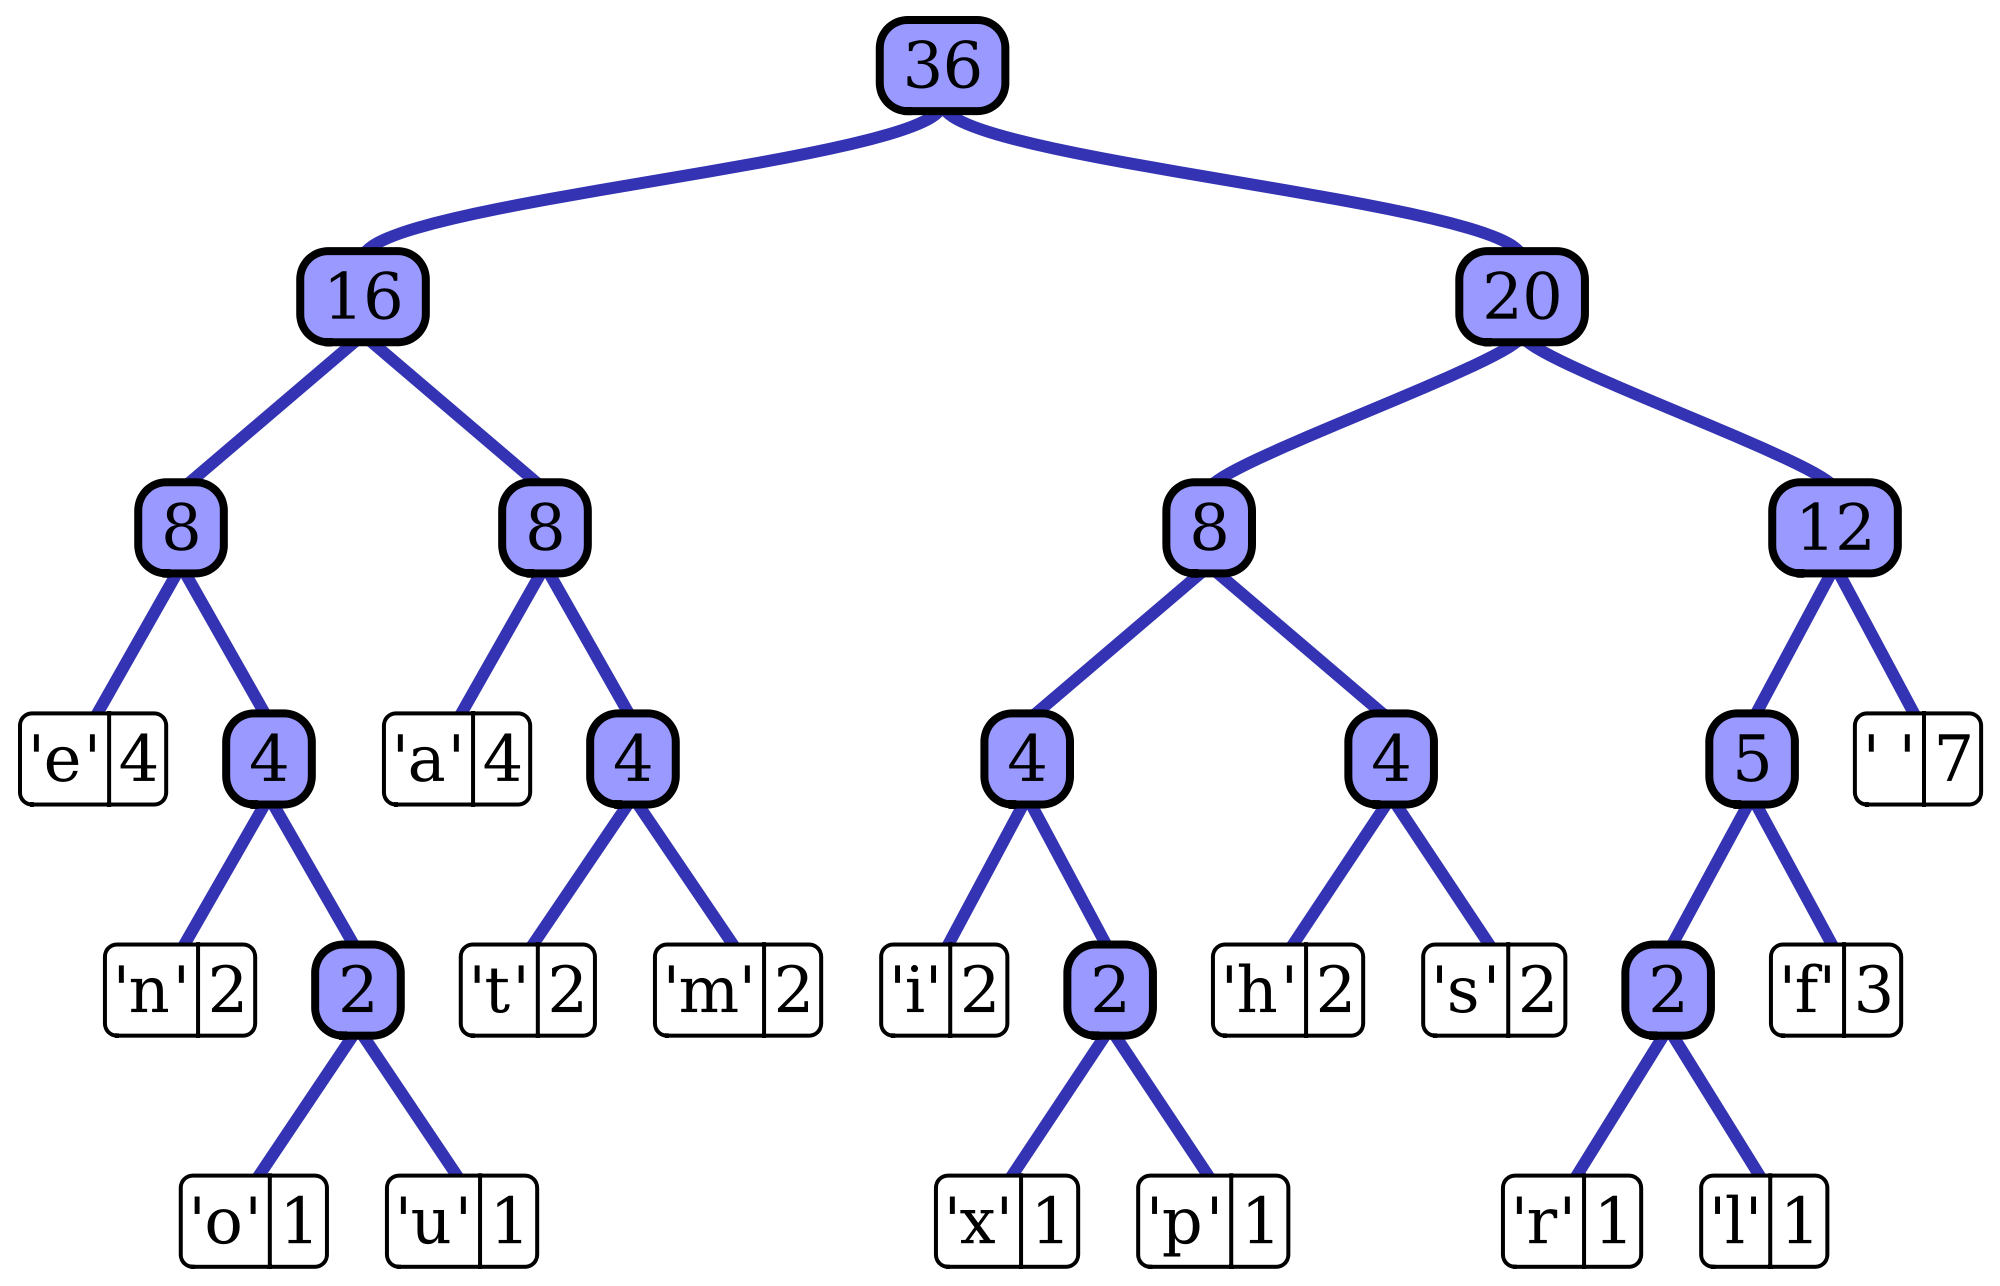
\includegraphics[width=\linewidth]{Billeder/Huffman_tree_2.png}
\caption{Huffman tr�}
\label{fig:huffmantree}
\end{figure}

\begin{table}
\begin{tabular}{|c|c|c|}
\hline
Tegn & Hyppighed & Bin�r kode \\
\hline \hline
space & 7 & 111 \\ 
\hline 
a & 4 & 010 \\ 
\hline 
e & 4 & 000 \\ 
\hline 
f & 3 & 1101 \\ 
\hline 
h & 2 & 1010 \\ 
\hline 
i & 2 & 1000 \\ 
\hline 
m & 2 & 0111 \\ 
\hline 
n & 2 & 0010 \\ 
\hline 
s & 2 & 1011 \\ 
\hline 
t & 2 & 0110 \\ 
\hline 
l & 1 & 11001 \\ 
\hline 
o & 1 & 00110 \\ 
\hline 
p & 1 & 10011 \\ 
\hline 
r & 1 & 11000 \\ 
\hline 
u & 1 & 00111 \\ 
\hline 
x & 1 & 10010 \\ 
\hline 
\end{tabular}
\caption{Hyppighed og kode af forskellige tegn}
\label{tab:huffmantable}
\end{table}